\documentclass[11pt]{article}
\renewcommand*\familydefault{\sfdefault}
%\usepackage{amssymb,amsmath,amsfonts,comment}
%\usepackage{amsmath,amssymb,graphicx,subfigure,psfrag}
\usepackage{amsmath,amssymb,graphicx,subfigure,psfrag,upgreek}
\usepackage{amssymb,mathrsfs}
\usepackage[margin=1in]{geometry}
\usepackage{tikz,pgfplots,graphicx}
\usepackage{color,pdfcolmk}
\usepackage{amsmath}
%\usepackage{subcaption}

%\newcommand{\alennote}[1]{\noindent\emph{\textcolor{blue!50!black}{Alen:#1\:}}}
%\newcommand{\gsnote}[1]{\noindent\emph{\textcolor{green}{GS: #1\:}}}
\newcommand{\todo}[1]{\noindent\emph{\textcolor{red}{Todo: #1\:}}}
\newcommand{\note}[1]{\noindent\emph{\vspace{1ex}\textcolor{blue}{Note: #1\:}}\\[1ex]}
\newcommand{\nnote}[1]{\noindent\emph{\vspace{1ex}\textcolor{red}{Note: #1\:}}}
\newcommand{\referee}[1]{\vspace{.1ex}\noindent{\textcolor{blue}{#1}}}
\newcommand{\nnn}{\mathbf{n}}
\newcommand{\fff}{\mathbf{f}}
\newcommand{\uuu}{\mathbf{u}}
\newcommand{\+}{\otimes}
\newcommand{\m}{\mathcal}
\newcommand{\bs}[1]{\ensuremath{\boldsymbol{#1}}}
\newcommand{\eps}{\varepsilon}


\newcommand{\gs}[1]{\textcolor{green}{G: #1}}
\newcommand{\np}[1]{\textcolor{blue}{N: #1}}
\newcommand{\tuck}[1]{\textcolor{brown}{T: #1}}
\newcommand{\mauro}[1]{\textcolor{red}{#1}}



\begin{document}

\section*{Reply to the Reviewer 1:}

Thanks for the careful reading and for your helpful comments and
suggestions.  Please find below point-by-point replies (in black) to
your comments and questions (which are reprinted in blue). To give you
an overview of all the changes in the paper, we also provide a
diff-document that highlights the changes between the initial
submission and this re-submission.\\[1ex]

\referee{Many Hessian-based computational algorithms have been
  developed to solve large-scale inverse problems constrained by
  partial differential equations (PDEs) in the last decade, especially
  in the context of inferring infinite-dimensional
  parameters. However, it remains a critical computational challenge
  to solve such inverse problems when the Hessian of the data-misfit
  term does not have fast spectrum decay, or the Hessian is
  high-rank. This challenge often leads to the need to solve a
  considerable number of PDEs in many (preconditioned) CG iterations
  with an inexact Newton-CG algorithm, one of the most advanced
  optimization algorithms in solving infinite-dimensional inverse
  problems.\\}

  \referee{To address this challenge, this paper proposes an
  efficient preconditioned CG method with the preconditioner computed
  as an approximate Hessian at some suitable parameter point, which is
  demonstrated to significantly reduce the number of required CG
  iterations to achieve given accuracy. The key novelty of this paper
  is the development of an efficient hierarchical matrix approximation
  of the Hessian using only a small number of Hessian matrix-vector
  products, thus a small number of PDE solves. This novelty is made
  possible by exploiting the property of the Hessian operator with
  locally supported non-negative integral kernels. Specifically, the
  authors propose a point spread function (PSF) approximation of the
  Hessian by (1) computing the zeroth, first, and second-order
  impulse response moments of the Hessian by applying its product with
  constant, linear, and quadratic functions, (2) building local
  ellipsoid support es- timate of the impulse response functions of
  the Hessian based on these moments, (3) selecting sample points of
  the impulse response from a candidate set by a greedy ellipsoid
  packing algorithm, (4) computing the impulse responses with disjoint
  ellipsoid in batches by applying the Hessian to Dirac combs, which
  plays a key role in reducing the total number of Hessian
  matrix-vector product, (5) approximating any integral kernel entries
  by a radial basis interpolation based on the computed impulse
  responses, and (6) building the hierarchical matrix approximation of
  the Hessian with the radial basis interpolation of the integral
  kernel entries before applying proper symmetrizing and flipping of
  the negative eigenvalues to make the approximate matrix symmetric
  positive semi-definite.\\}

\referee{The PSF approximation in this paper is built for more general
  operators than Hessian. It demonstrates the effectiveness of the
  PSF-based method by 1 using it to build preconditioners for the
  Hessian operator in two challenging inverse problems of basal
  friction coefficient inversion of ice sheet flow and ini- tial
  condition inversion of advection-dominated transport. It shows
  significant reductions (5-10X) in the required number of PDE solves
  compared to classical regularization-based preconditioning and no
  preconditioning. The paper also presents a comprehensive numerical
  study on the influence of various parameters (data noises, \# batchs,
  diffusion coefficients, terminal times) on the effective- ness and
  data-scalability of the proposed method, showing that the PSF-based
  preconditioners can form good approximations of high-rank Hessians
  using only a small number of operator applications.  The proposed
  method is very interesting and makes a great contribution to solving
  large-scale inverse problems with high-rank Hessians. The
  presentation of the proposed method is concise and illustrative. The
  numerical results are very convincing. Overall, the paper is very
  well written.\\}

\noindent{Thank you for the positive assesment of our work.\\}

\paragraph{General Comments:}

\referee{I recommend to accept the paper for publication with minor
  revisions. I suggest the authors properly address the following
  questions to help for its better understanding and broader
  applications.\\}



\begin{enumerate} 
\item \referee{The author mentioned one limitation of the proposed method:
      the Hessian should have a local non-negative integral kernel,
      which is not satisfied for wave inverse problems that lead to a
      substantial amount of negative entries of the Hessian. It would
      be interesting if the author could elaborate more details with
      intuition or numerical evidence for this property and the
      limitation, especially if you also use Gauss-Newton approximate
      Hessian for the wave inverse problems as in this paper.}

\noindent{
	We added a numerical study investigating the robustness of the method to violations of the non-negative kernel assumption on two two-dimensional blurring kernel examples (Figure 7). We also added a discussion of the impact of non-locality and negativity on the performance of the method (Section 3.2).
	
	One takeaway message from Figure 7 is that the impact of negative numbers depends strongly on the spatial configuration of these negative numbers---in the first example (columns~1 and~2 in Figure~7), the negative numbers have minimal impact on the ellipsoid impulse response support estimates, whereas in the second example (columns~3 and~4), even a small amount of negative numbers causes the impulse response support estimate to be poor. The configuration of negative numbers for the integral kernel in wave inverse problem Hessians (including Gauss-Newton Hessians) is similar to that of the second example, and therefore our method is unlikely to be effective for wave Hessians. 
	
	Although the component of the wave inverse problem Hessian corresponding to reflected waves is local, the component corresponding to transmission waves is non-local, which also poses challenges for our method (as discussed in the revised version of Section 3.2). If one applied a high-pass filter to remove the transmission component, in principle the impulse responses could be localized. However, the non-negativity would still need to be addressed. 
	
	In Figure \ref{fig:marmousi_impulse} here (but not in the paper due to page limitations), we show an impulse response for the Gauss-Newton Hessian for the Marmousi wave inverse problem. Note that the non-local component of the impulse response shifts the mean far away from the visual ``center'' of the impulse response, and causes the ellipsoid impulse response support estimate to be effectively the entire domain.
	
	We also added more references and discussion regarding the wave inverse problem Hessian at the end of Section 2 in the revised manuscript.
	
	\begin{figure}
		\centering
		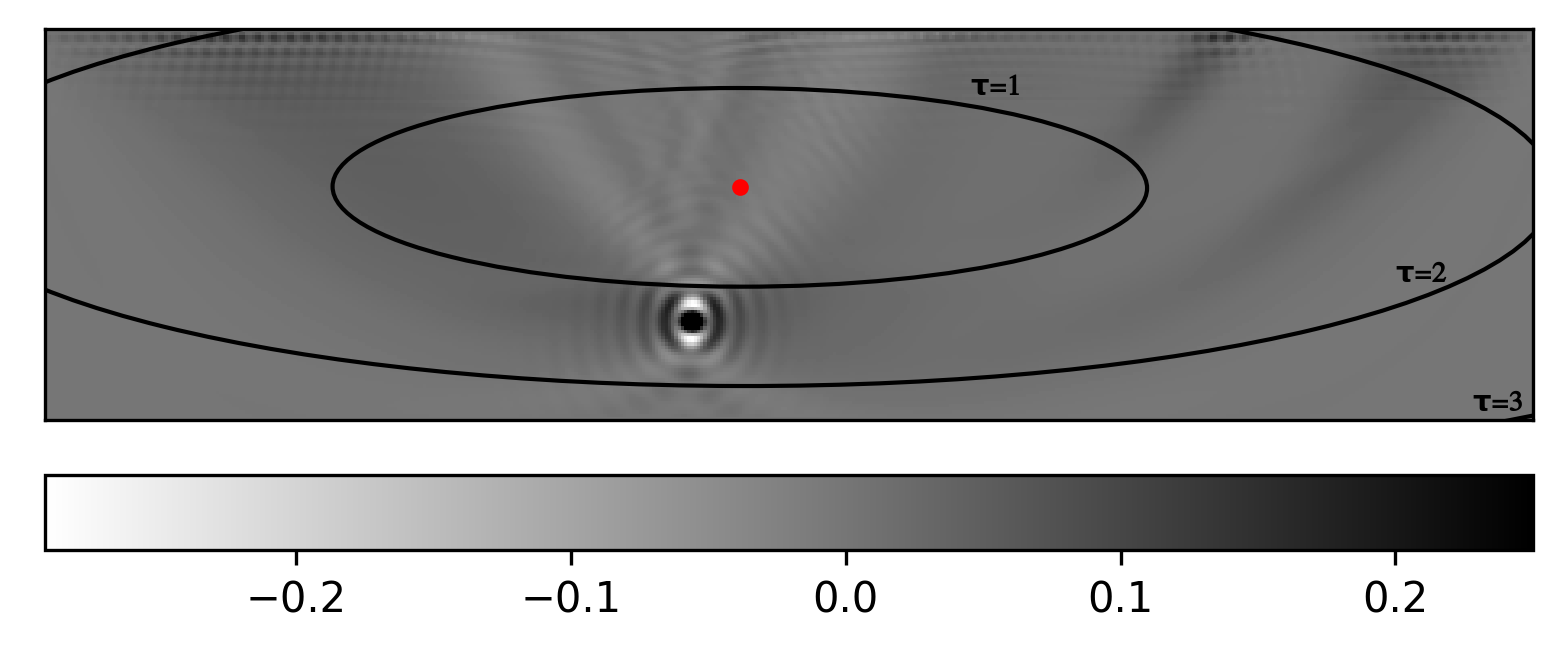
\includegraphics[scale=0.735]{marmousi_impulse_response_full_domain_ellipsoid_with_tau_annotations.png}
		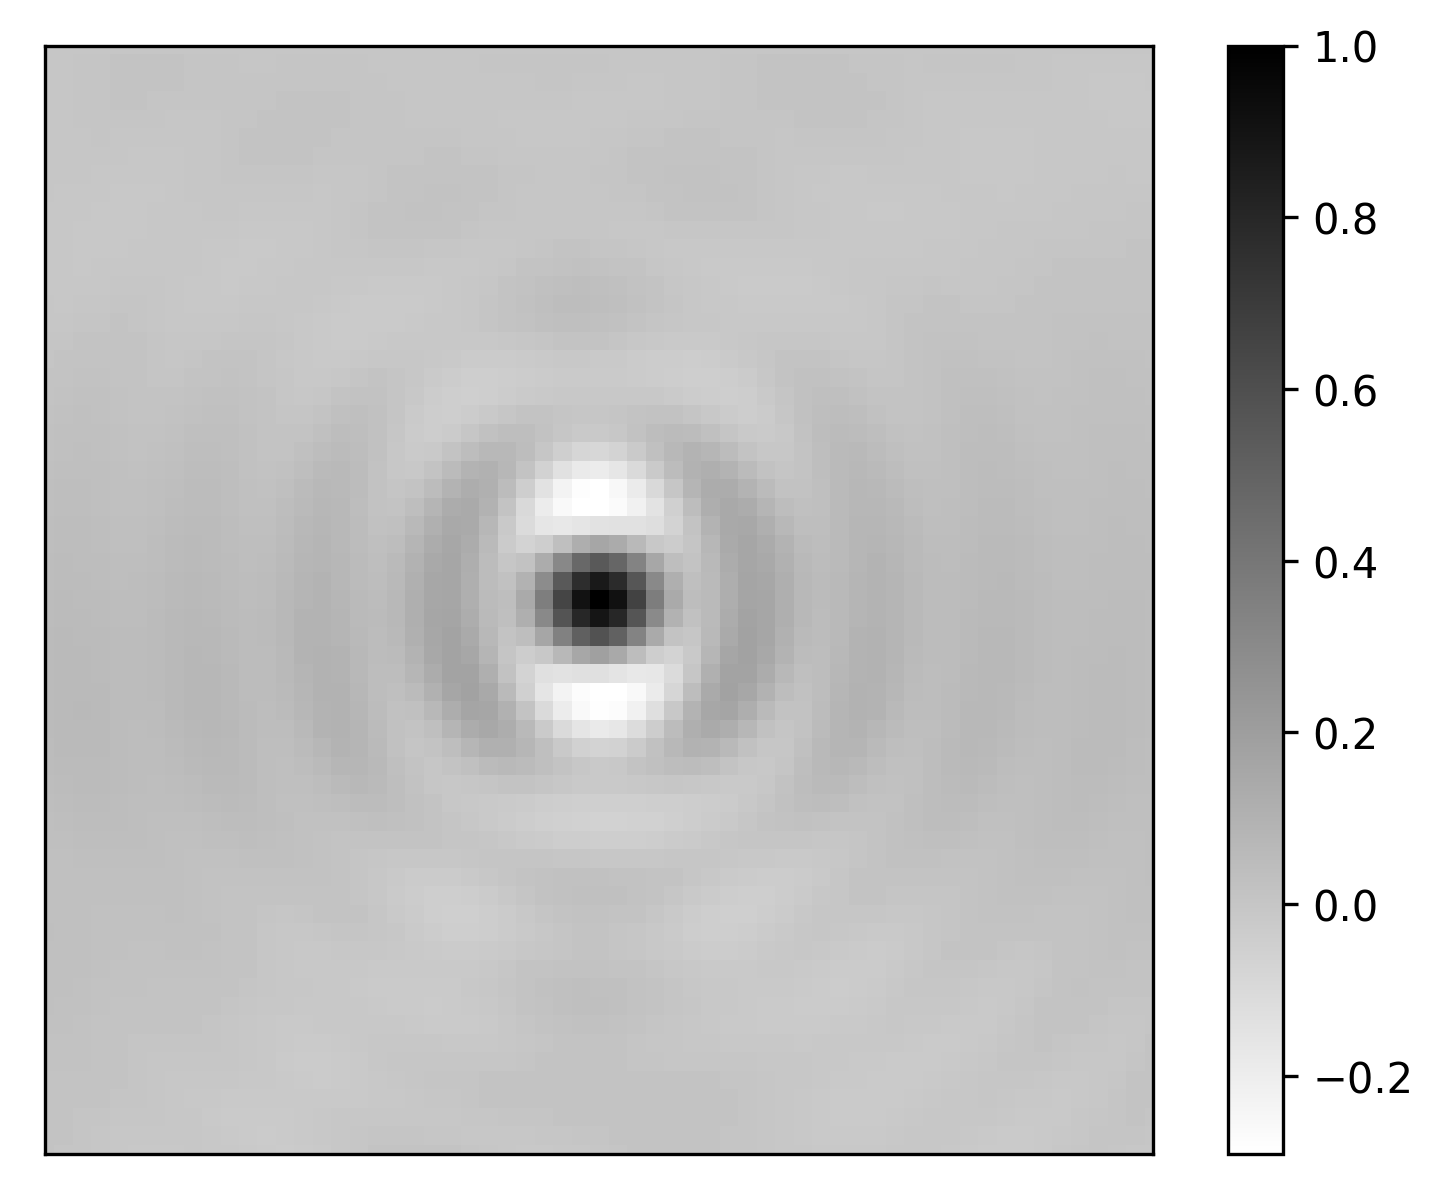
\includegraphics[scale=0.3975]{marmousi_impulse_response_zoomed_in.png}
		
		\caption{Impulse response for the Gauss-Newton Hessian for the Marmousi wave inverse problem. On the left we show the impulse response on the whole domain. The color scale is truncated for better visualization of the non-local transmission components. The estimated mean of the impulse response is shown as a red dot. Estimated support ellipsoids with $\tau\in \{1.0, 2.0, 3.0\}$  are shown as black ellipses. On the right we show a zoomed in impulse response, showcasing the negative numbers in the integral kernel. The data for this impulse response was kindly provided to us by Mathew Hu (UT Austin).
		}
		\label{fig:marmousi_impulse}
	\end{figure}
	
%	Perhaps this issue could be addressed by applying a high-pass filter to remove the non-local transmission component.
%	 The transmission component is typically low rank and can therefore be addressed with other methods. 
%	We do not pursue this here.
	
%	NICK ADD PLOT
%	
%	In particular, we note the poor performance for the Ricker wavelet-type kernel (right two columns of Figure 7). We observed a similar configuration for the impulse responses for the Hessian and Gauss-Newton Hessian in wave inverse problems. 
	

	
%	 The configuration of negative numbers in this example is similar The negative numbers in the integral kernel for the wave Hessian (and Gauss-Newton Hessian) are distributed in a manner similar to the Ricker wavelet-type impulse response shown in the right two columns of Figure 7.
%	
%	 We also added a discussion of the impact of non-locality and negativity on the performance of the method (Section 3.2).
%	
%	The 
%	
%	(1) Three-figure plot: Stokes, Advection/diffusion, wave impulse responses. 
%	
%(2) showing that the method performs poorly for the ricker example
%	
%Nick will try to get an impulse response for the wave
%  problem.
}

\item \referee{It is interesting to see the effectiveness of the
  approximate Hessian used as a preconditioner. It would also be very
  interesting to see how accurate the approximate Hessian is compared
  to a full Hessian in terms of the number of batches, ellipsoid
  sizes, and in particular the total number of impulse responses. Can
  you say anything about the convergence of the approximation, either
  numerical or theoretical?}

  \noindent{
  	In Figure 8 in the revised manuscript we added a convergence study for one of the blur kernel examples. We show the convergence of the proposed PSF method as a function of the total number of impulse responses and the number of batches, for several ellipsoid size parameters $\tau$ ranging from $2.0$--$4.0$. We observe a roughly linear convergence rate until a limit, which depends on $\tau$, is reached. The larger $\tau$ is, the smaller the limit is on the achievable error. Before this limit, the error decreases at roughly the same rate for all $\tau$ in terms of the number of impulse responses. This means that the error decreases faster for smaller $\tau$ as a function of the number of batches, since smaller $\tau$ means more impulse responses per batch. Basically, with larger $\tau$ the method converge more slowly than with smaller $\tau$, but larger $\tau$ allows the method to eventually achieve a lower level of error. We added a discussion of this convergence study in Section 7.1 of the revised manuscript.
  	
  	Although the method can achieve high accuracy, we would like to emphasize that it is targeted at achieving modest accuracies (e.g., $5\%$ error) to build preconditioners for problems that are challenging for existing methods. In Table 2 in the revised manuscript, following the other reviewer's suggestion, we added a comparison of the computational cost
  	(measured in operator applies) to approximate the kernel in one of the spatially
  	varying blurring kernel examples. We compare the results using the proposed PSF method,
  	the randomized HODLR (hierarchical off diagonal low rank) method,
  	and GLR (global low rank) approximation using randomized SVD. The
  	results show an overwhelming computational gain.
  	
%  	 I.e., the relative error decreases as $\text{constant} \times \left(\# \text{impulse responses}\right)^{-1}$ or $\text{constant} \times \# \text{batches}^{-1}$ until the limit is reached, then the error does not decrease any further. Increasing $\tau$ lowers this limit, allowing the method to achieve higher accuracy. Before this limit is reached, the convergence rate is the same for all $\tau$ as a function the number of impulse responses. 
  	
%  	Figure 6 illustrates how the error decreases with increasing numbers of batches and therefore impulse responses. ALSO TABLE 4 CONDITION NUMBER
%  	
%  	Frog example with a=1. Error vs \#batches, for different tau. Also do a plot with \#impulses on the x-axis.
%  	
%  	Nick will try to create a plot that shows some error
%    (e.g. Frob norm, cond number) as a function of number of impulse
%    responses.
}

 \item \referee{The paper presented a nice complexity analysis of the
   steps in constructing the approximate Hessian, with the dominating
   cost arising from the Hessian matrix-vector product. It would be
   interesting to see the computational time of each step for the
   numerical examples to provide a good sense of the complexity and to
   support the 5--10X computational reduction by accounting also the
   overhead beyond the PDE solves.
}

   \noindent{This is a fair point. We agree with the reviewer that there is an overhead
     beyond the PDE solves. However, since we have not optimized our codes for performance, it would be
     perhaps misleading to report profiling/timing information. Nevertheless, for all numerical tests we
     present in this paper, the cost to build the H-matrices (item (2) in Section 6) was small compared to
     PDE solves (item (1) in Section 6). The further H-matrix linear algebra operations (item (3) in Section 6), as implemented in the HLIBPro library, were less costly than the PDE solves, but their costs were not negligible. In particular, enforcing positive definiteness of the H-matrix via the procedure presented in Section 5.5 was costly. Because of the polylog linear complexity of H-matrix operations, for large-scale problems these H-matrix overhead costs would eventually become insignificant compared to the PDE solves.
%     
%     However, for all numerical tests we
%     present in this paper, this cost was small compared to
%     PDE-applies. This is due to the need for a relatively small
%     number of sample points ($m$) in all batches. Since we have not
%     invested time to optimize our codes for performance, it would be
%     perhaps misleading to report profiling-timing information. When
%     $m$ is very large, one can reduce this cost with more involved
%     computational geometry methods. This was beyond the scope of our
%     work.
}
   
\end{enumerate} 

%\bibliographystyle{unsrt}
%\bibliographystyle{iopart-num}
%\bibliography{reviewer2_references}

\end{document}
